\documentclass{beamer}
\usepackage[T1]{fontenc}
\usepackage{multicol}
\usepackage{ragged2e}   %new code
\usepackage[utf8]{inputenc}
\usepackage[brazil]{varioref}
\usepackage[square,sort,comma,super,authoryear]{natbib}
\usepackage{xmpmulti}
\usepackage{epsfig}
\usepackage{subcaption}
\captionsetup{compatibility=false}
\usepackage{ru,graphicx,hyperref,url} %

\addtobeamertemplate{block begin}{}{\justifying}
\setbeamertemplate{section in toc}[sections numbered]
\AtBeginSection[]
{
  \begin{frame}{Índice}
  \begin{multicols}{2}
      \tableofcontents[currentsection]
    \end{multicols}
  \end{frame}

}

% The title of the presentation:
%  - first a short version which is visible at the bottom of each slide;
%  - second the full title shown on the title slide;

\title[Perfil étnico-racial ]{
Perfil étnico-racial dos estudantes da Universidade Estadual de Maringá: \\ Um olhar para o Departamento de Estatística}

% Optional: a subtitle to be dispalyed on the title slide
% \subtitle{Show where you're from}

% The author(s) of the presentation:
%  - again first a short version to be displayed at the bottom;
%  - next the full list of authors, which may include contact information;
\author[A VIDA É BELA!!!]{
  Lucas Stefano Xavier de Sousa\\
  Luiz Otavio Rodrigues Mendes\\
  Paulo Vinícius Moreira da Costa Menezes\\
  Maurício Tatsuo Emori\\\medskip
  {\small {Prof Dr. Diego Correa Alves}
  }}

% The institute:
%  - to start the name of the university as displayed on the top of each slide
%    this can be adjusted such that you can also create a Dutch version
%  - next the institute information as displayed on the title slide
\institute[Universidade Estadual de Maringá ]{
  Departamento de Estatística - UEM \\}

% Add a date and possibly the name of the event to the slides
%  - again first a short version to be shown at the bottom of each slide
%  - second the full date and event name for the title slide
\date{\today}

\begin{document}

\begin{frame}
  \titlepage
\end{frame}

% Section titles are shown in at the top of the slides with the current section 
% highlighted. Note that the number of sections determines the size of the top 
% bar, and hence the university name and logo. If you do not add any sections 
% they will not be visible.
\section{Motivação}
\subsection{O que nos motivou?}

\begin{frame}
    \frametitle{O que nos motivou?}
    \framesubtitle{Motivação}
    \justifying
    \\
    Acreditamos que uma análise crítica abordando um tema tão relevante como este se faz necessária, em especial em uma época em que o debate público e a mídia vem pautando diversos acontecimentos envolvendo as questões étnicas-raciais.\\
    \\Ainda, esta constitui uma oportunidade para o grupo sair de sua "zona de conforto", buscando aprender e se familiarizar com um tema desconhecido pelos mesmos.
    
\end{frame}

%%%CONTEXTO%%%
\subsection{Dados Históricos}

\begin{frame}
    \frametitle{Dados Históricos}
    \framesubtitle{Motivação}
    \justifying

    Segundo o censo mais recente, de 2010, do IBGE - Instituto Brasileiro de Geografia e Estatística:
    \begin{figure}
       \centering
       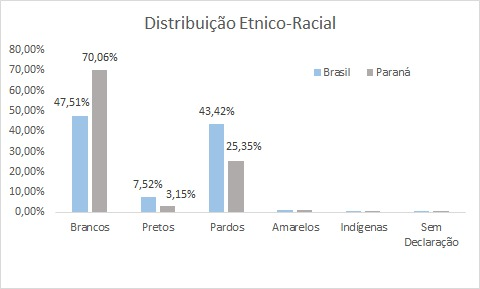
\includegraphics[width=8.5cm]{distribuicao-etnico-racial.jpeg}
   \end{figure}
    
    
\end{frame}

%%%%CONTEXTO ATUALS%%%%
\subsection{Contexto Atual}

\begin{frame}
    \frametitle{Contexto Atual}
    \framesubtitle{Dados da UEM}
    \justifying
   De acordo com os últimos dados disponibilizados pela CVU-UEM (Comissão de Vestibular Unificado), nota-se que as proporções vistas no censo de 2010 não eram semelhantes às encontradas na UEM no ano de 2010, como mostra o gráfico abaixo:
   \begin{figure}
       \centering
       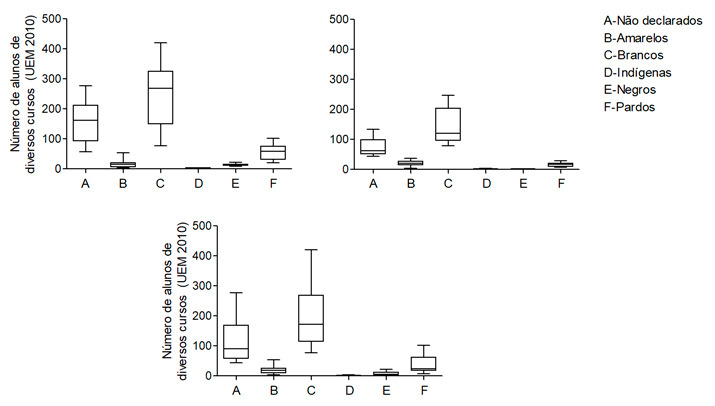
\includegraphics[width=7.1cm\textwidth]{grafico04.jpeg}
       \caption*{FONTE: (Neves et al., 2012)\small}
   \end{figure}
    
\end{frame}

\subsection{Contexto Atual}

\begin{frame}
    \frametitle{Dados da UEM}
    \framesubtitle{Contexto Atual}
    \justifying
   Em 2014, foi aprovada a lei 12.990 que institui as cotas raciais nos concursos públicos. Essa medida teve implicações imediatas nas proporções étnico-raciais dos alunos da UEM, mostradas no gráfico a seguir:
    \begin{figure}
       \centering
       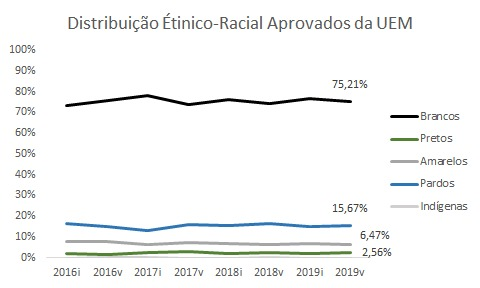
\includegraphics[width=8.1cm]{grafico-linhas-cotas.jpeg}
   \end{figure}
   
\end{frame}

%%%%METODOLOGIA%%%%
\subsection{Objetivo}

\begin{frame}
    \frametitle{Objetivo}
    \framesubtitle{Motivação}
    \justifying
    \begin{itemize}
        \item Desvelar o perfil étnico-racial dos estudantes da Universidade Estadual de Maringá nos últimos 5 anos;
        \item Analisar o perfil étnico-racial dos estudantes do curso de Bacharelado em Estatística;
    \end{itemize}

\end{frame}

\section{Metodologia}
\begin{frame}{Metodologia}

           \begin{itemize}
    \item Coleta dos dados;
           \item Relatórios e dados brutos advindos da UEM;
            \item Questionário com perguntas fechadas a ser enviado a todos os estudantes do curso de Estatística;
              \end{itemize}
\begin{itemize}

    \item Análise quantitativa dos dados por meio de:
        \item  Estatística descritiva;
        \item  Correlação de dados.

\end{itemize}

\end{frame}

\section{Considerações Finais}
\subsection{Considerações Finais}
\begin{frame}{O que esperamos?}
\framesubtitle{Considerações Finais}
    \justifying
  \\
Acreditamos que os objetivos desta pesquisa ao serem alcançados podem propiciar um panorama dos estudantes do Departamento de Estatística da UEM.\\
\\Assim, tais resultados podem colaborar na discussão sobre o tema e possibilitar que melhores políticas públicas sejam tomadas em relação às minorias étnico-raciais.

\end{frame}

\section{Referências}
\subsection{Referências}
\begin{frame}{Referências}
\framesubtitle{Referências}
    \justifying
NEVES, Pedro Dias Mangolini; DE LIMA, Maria das Graças; DOS SANTOS, Aldenir Dias. Onde estão os alunos negros da Universidade Estadual de Maringá (PR)?. Revista da Associação Brasileira de Pesquisadores/as Negros/as (ABPN), v. 3, n. 7, p. 117-127, 2012.

\end{frame}
\begin{frame}[plain,c]
   \begin{figure}
       \centering
       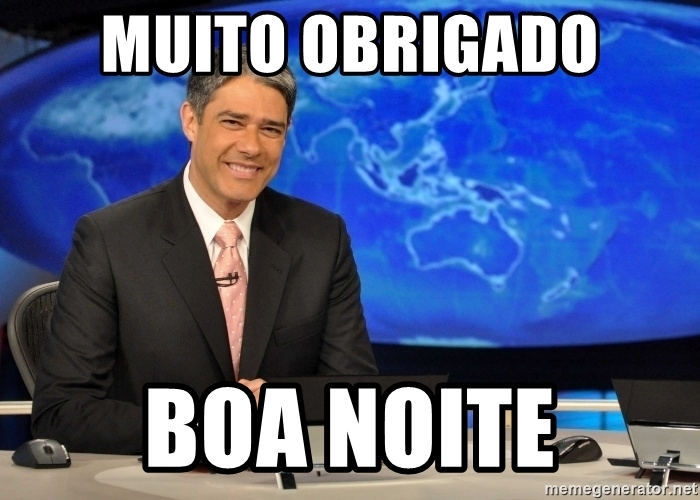
\includegraphics[width=10cm]{bonner.jpg}
   \end{figure}
\end{frame}

\end{document}